\scanpage{86}
\mspage{- 541 -}

\noindent\qquad 3.8. Morphismes universellement ouverts , universellement fermés , universellement bicontinus\dotfill

\noindent\qquad 3.9. Morphismes générisants\dotfill

\noindent\qquad 3.10. Morphismes submersifs et universellement submersifs

\noindent\quad \S\ 4. Sous-schémas et morphismes d'immersion .\makebox[0pt][l]{\hspace{0.35em}\raisebox{-0.5ex}[0pt][0pt]{\parbox[c]{1mm}{\figure{\unsure{%
\begin{tikzpicture}[x=1mm,y=1mm,baseline=0pt]
\fill (0,0) ellipse[x radius=0.13,y radius=0.22,rotate=-30];
\end{tikzpicture}%
}}}}} Schémas réduits\dotfill

% Faint unassigned vertical trace between the preceding leaders and the 4.1 leaders.
% Material/writing status is uncertain; no handwritten attribution is asserted.
\noindent\makebox[0pt][l]{\hspace{0.42\linewidth}\raisebox{-0.7ex}[0pt][0pt]{\parbox[c]{2mm}{\figure{\unsure{%
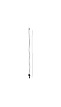
\begin{tikzpicture}[x=1mm,y=1mm,baseline=0pt]
\draw[gray!55,line width=0.25pt] (0.05,6.4)
 .. controls (-0.05,5.7) and (0.18,5.3) .. (0.10,4.8)
 .. controls (0.18,4.3) and (-0.05,3.8) .. (0.08,3.3)
 .. controls (0.25,2.9) and (-0.04,2.5) .. (0.08,2.0)
 .. controls (0.19,1.6) and (0.09,1.0) .. (0.06,0.55);
\draw[gray!30,line width=0.18pt] (0.48,6.2)
 .. controls (0.36,4.2) and (0.54,2.2) .. (0.44,0.15);
\fill[gray!80] (0.01,6.5) -- (0.19,6.35) -- (0.03,6.18) -- cycle;
\fill (0.03,0.62) .. controls (-0.13,0.52) and (-0.06,0.40) .. (0.08,0.35)
 .. controls (0.19,0.30) and (0.25,0.42) .. (0.15,0.52) -- cycle;
\draw[line width=0.22pt] (0.10,0.32) -- (0.12,0.05);
\end{tikzpicture}%
}}}}}\qquad 4.1. Sous-schémas\dotfill

\noindent\qquad 4.2. Morphismes d'immersion\dotfill

\noindent\qquad 4.3. Image réciproque d'un sous-schéma\dotfill

\noindent\qquad 4.4. Immersions locales et isomorphismes locaux\dotfill

\noindent\qquad 4.5. Schémas réduits\dotfill

\noindent\qquad 4.6. Existence d'un sous-schéma d'espace sous-jacent donné\dotfill

\noindent\quad \S\ 5. Morphismes séparés . Critères valuatifs\dotfill

\noindent\qquad 5.1. Diagonale d'un $S$-schéma\dotfill

\noindent\qquad 5.2. Morphismes et schémas séparés\dotfill

\noindent\qquad 5.3. Critères \deleted{\unsure{a|e}}de séparation\dotfill

\noindent\qquad 5.4. Morphismes schématiquement dominants et sous-schémas schématiquement denses\dotfill

\noindent\qquad 5.5. Critères valuati\deleted{\unsure{s|b}}fs\dotfill

\noindent\quad \S\ 6. Conditions de finitude relatives\dotfill

\noindent\qquad 6.1. Morphismes quasi-compacts et morphismes quasi-séparés\dotfill

\noindent\qquad 6.2. Morphismes localement de type fini et morphismes localement de présentation finie\dotfill

% Two unassigned points lie above the right-hand part of the 6.3 leaders.
\noindent\qquad 6.3. Morphismes de type fini et morphismes de présentation finie\dotfill\makebox[0pt][l]{\hspace{-0.08\linewidth}\raisebox{1.5ex}[0pt][0pt]{\parbox[c]{2mm}{\figure{\unsure{%
\begin{tikzpicture}[x=1mm,y=1mm,baseline=0pt]
\fill (-0.15,-0.05) .. controls (-0.18,0.12) and (-0.05,0.20) .. (0.05,0.14)
 .. controls (0.11,0.10) and (0.16,-0.04) .. (0.10,-0.09) -- cycle;
\fill (0.48,0.68) ellipse[x radius=0.13,y radius=0.20,rotate=-30];
\end{tikzpicture}%
}}}}}

\noindent\qquad 6.4. Schémas de \deleted{d}Jacobson et anneaux de \deleted{j}Jacobson\dotfill

\noindent\qquad 6.5. Schémas algébriques et localement algébriques\dotfill

\noindent\qquad 6.6. Détermi\deleted{j}nation locale d'un morphisme\dotfill

\noindent\qquad 6.7. Image directe d'un faisceau quasi-cohérent\dotfill

\noindent\qquad 6.8. Prolongement de sections de faisceaux quasi-cohérents

\noindent\qquad 6.9. Prolongement des faisceaux quasi-cohérents\dotfill

\noindent\qquad 6.10.Image schémat\deleted{\unsure{l|t}}i\makebox[0pt][l]{\hspace{-0.25em}\raisebox{-1.0ex}[0pt][0pt]{\parbox[c]{1.4mm}{\figure{\unsure{%
\begin{tikzpicture}[x=1mm,y=1mm,baseline=0pt]
\fill (0,0) ellipse[x radius=0.09,y radius=0.10];
\fill (0.25,0.01) .. controls (0.36,0.12) and (0.47,0.10) .. (0.53,0.03)
 .. controls (0.64,0.13) and (0.75,0.07) .. (0.73,-0.02)
 .. controls (0.58,-0.08) and (0.38,-0.13) .. (0.25,0.01) -- cycle;
\end{tikzpicture}%
}}}}}que d'un schéma\unsure{,|.} Adhérence schématique d'un sous-schéma\dotfill

\noindent\qquad 6.11.Morphismes quasi-finis\dotfill

% archive sheet number: 85
